\documentclass{article}[12 pt]

\usepackage{fancyhdr}
\usepackage{extramarks}
\usepackage{amsmath}
\usepackage{float}
\usepackage{graphicx}
\usepackage{subcaption}
%
% Basic Document Settings
%

\topmargin=-0.45in
\evensidemargin=0in
\oddsidemargin=0in
\textwidth=6.5in
\textheight=9.0in
\headsep=0.25in

\linespread{1.1}

\pagestyle{fancy}
\lhead{\hmwkAuthorName}
\chead{\hmwkTitle}
\lfoot{\small{\hmwkAuthorRoll}}
\cfoot{\thepage}

\renewcommand\headrulewidth{0.4pt}
\renewcommand\footrulewidth{0.4pt}

\setlength\parindent{0pt}



%
% Homework Details
%   - Title
%   - Due date
%   - Class
%   - Instructor
%   - Author
%

\newcommand{\hmwkTitle}{Communication 1 System Assignment\#1}
\newcommand{\hmwkDueDate}{August 30, 2020}
\newcommand{\hmwkClassInstructor}{Lecturer: Suman Sharma}
\newcommand{\hmwkAuthorName}{\textbf{Ashlesh Pandey}}
\newcommand{\hmwkAuthorRoll}{\textbf{PUL074BEX007}}
%
% Title Page
%

\title{
    \vspace{2in}
    \textmd{\textbf{\hmwkTitle}}\\
    \normalsize\vspace{0.1in}\small{Due\ on\ \hmwkDueDate}\\
    \vspace{0.1in}\large{\textit{\hmwkClassInstructor}}
    \vspace{3in}
}

\author{
    \textmd{\textbf{\huge{\hmwkAuthorName}}}\\ \\
    \textbf{\huge{\hmwkAuthorRoll}}
}
\date{}

%
% Various Helper Commands
%


% Alias for the Problem section header
\newcommand{
\problem}[2]
{\textbf{\huge Problem {#1} \\
\normalsize {#2}\\
}
}

% Alias for the Solution section header
\newcommand{\solution}{
\large{\textit{Solution}}
}

\begin{document}
\pagenumbering{gobble}
\maketitle
\pagebreak
\pagenumbering{arabic}
\problem{1}{Determine $v(t)*w_1(t)$ and $v(t)*w_2(t)$. Show your work graphically and mathematically. Given that
$v(t)=e^{-t}u(t)$, 
$w_1(t)=\delta(t)$,  
$w_2(t)=\delta(t-10)$.}
\solution
\subsection*{Mathematical approach}
The convolution of two functions, say, $y(t)=x(t)*h(t)$ is given by:
\begin{equation}
y(t)=x(t)*h(t)=h(t)*x(t)=\int_{-\infty}^\infty x(\tau)h(t-\tau)d\tau
\end{equation}
Also, the dirac(delta) function has a special integration property that we'll use to easily calculate the integration, the property being,
\begin{equation}
\int_{-d}^{d} f(t) \delta(t-a)dt=f(a)
\end{equation}
such that $-\infty \leq -d < a < d \leq \infty$.\\ Likewise, since $d(t)$ is an even function the following equation holds true.
\begin{equation}
\delta(t)=\delta(-t)
\end{equation}

Mathematically,
\begin{equation}
v(t)*w_1(t)=\int_{-\infty}^\infty e^{-\tau}u(\tau)\delta(t-\tau)d\tau
\end{equation} 
and
\begin{equation}
v(t)*w_2(t)=\int_{-\infty}^\infty e^{-\tau}u(\tau)\delta((t-10)-\tau)d\tau
\end{equation} 
Using equation (3) to rearrange equation (4) and (5) we get,
\begin{equation}
v(t)*w_1(t)=\int_{-\infty}^\infty e^{-\tau}u(\tau)\delta(\tau-t)d\tau
\end{equation} 
and
\begin{equation}
v(t)*w_2(t)=\int_{-\infty}^\infty e^{-\tau}u(\tau)\delta(\tau-(t-10))d\tau
\end{equation} 
From the property of delta function mentioned in equation(2), equation(6) and (7) can be reduced to get,
\begin{equation}
v(t)*w_1(t)= e^{-t}u(t)
\end{equation} 
and
\begin{equation}
v(t)*w_2(t)=e^{-(t-10)}u(t-10)
\end{equation}
These equations are the solutions to the convolution problem obtained matematically.
\newpage
\subsection*{Graphical approach}
\begin{figure}[H]
\begin{subfigure}{.5\textwidth}
  \centering
  % include first image
  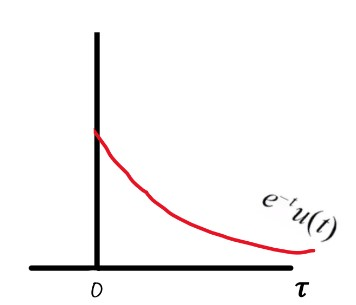
\includegraphics[width=.8\linewidth, height=.8\linewidth]{1.jpg}  
  \caption{Plot of $e^{-\tau}u(\tau)$ in $\tau$ axis}
  \label{fig:sub-first}
\end{subfigure}
\begin{subfigure}{.5\textwidth}
  \centering
  % include second image
  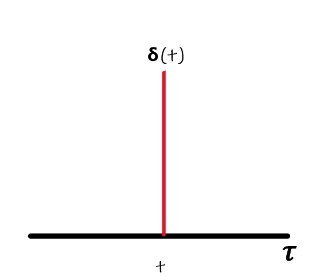
\includegraphics[width=.8\linewidth, height=.8\linewidth]{2.jpg}  
  \caption{Plot of $\delta(t)$ in $\tau$ axis}
  \label{fig:sub-second}
\end{subfigure}
\newline
\begin{subfigure}{\textwidth}
  \centering
  % include first image
  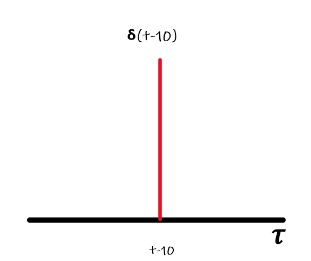
\includegraphics{3.jpg}  
  \caption{Plot of $\delta(t-10)$ in $\tau$ axis}
  \label{fig:sub-third}
\end{subfigure}
\newline
\begin{subfigure}{.5\textwidth}
  \centering
  % include first image
  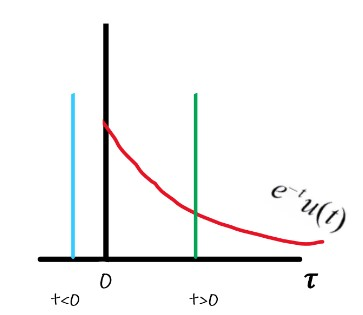
\includegraphics[width=.8\linewidth, height=.8\linewidth]{4.jpg}  
  \caption{Plot for $v(t)*w_1(t)$}
  \label{fig:sub-fourth}
\end{subfigure}
\begin{subfigure}{.5\textwidth}
  \centering
  % include second image
  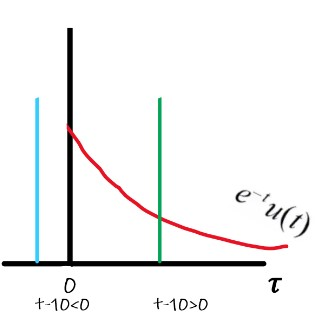
\includegraphics[width=.8\linewidth, height=.8\linewidth]{5.jpg}  
  \caption{Plot for $v(t)*w_1(t)$s}
  \label{fig:sub-fifth}
\end{subfigure}
\caption{Plot for calculating $v(t)*w_1(t)$ and $v(t)*w_2(t)$} 
\label{fig:fig}
\end{figure}
\newpage
Convolution of any two signals is simply the overlap of the signals represented all over the $\tau$ axis. So, figure(1 a), (1 b) and(1 c) show the three signals namely, $v(t)$,$w_1(t)$ and $w_2(t)$ in the $\tau$ axis. \\When the values of $t$ and $t-10$ in the respective figure (1 b) and (1 c) is either less than or greater than 0, the corresponding interaction with the $v(t)$ signal can be interpreted from the figure (1 d) and (1 e).\\\\
Both the signals $\delta(t)$ and $\delta(t-10)$ overlap with the signal $e^{-t}u(t)$ when they satisfy the condition, $t>0$ and $t-10>0$ respectively. This means the convolution of the signal $v(t)$ with $w_1(t)$ and $w_2(t)$ is nothing but the function $v(t)$ with $t=t$ and $t=t-10$ respectively, i.e. 
\begin{equation}
v(t)*w_1(t)=v(t)=e^{-t}u(t)
\end{equation} 
and
\begin{equation}
v(t)*w_2(t)=v(t-10)=e^{-(t-10)}u(t-10)
\end{equation}
\\\\ From this we can draw a conclusion that,
\begin{equation}
y(t)=x(t)*\delta(t \pm a)=x(t \pm a)
\end{equation}
\end{document}